\documentclass[titlepage,hidelinks,10pt]{article}
\usepackage[utf8]{inputenc}
\usepackage{parskip}
\usepackage[UKenglish]{babel}
\usepackage[headheight=15pt,margin=2cm]{geometry}
\usepackage{multicol}
\usepackage{multirow}
\usepackage[colorlinks=false]{hyperref}
\usepackage[super,square]{natbib}
\usepackage{float}
\usepackage[toc,page]{appendix}
\usepackage[table]{xcolor}
\usepackage{titling}
\usepackage{array}

\usepackage{color}
\usepackage{listings}
\usepackage{graphicx}
\graphicspath{ {img/} }
\usepackage{caption}
\usepackage{wrapfig}
\usepackage{lscape}
\usepackage{rotating}
\usepackage{epstopdf}
\usepackage{pifont}
\usepackage{gensymb}

\setlength{\parindent}{2em}

\date{January 2017}
\title{Augmented Reality Debugging System for Swarm Robotics \vspace{1cm}\\\Large{Initial Report}}
\author{Alistair Jewers}

\begin{document}

\maketitle

\tableofcontents
\newpage

\begin{multicols}{2}


\section{Project Overview and Aims}
Swarm Robotics is the name given to the nascent field of study focusing on the use of concepts derived from the study of social insect `swarms', such as ants or bees, to design and implement robot behaviours which allow a group of simple actors to achieve a complex, cooperative behaviour. The broader area of study, without the robotics focus, is referred to as Swarm Intelligence (SI), and is described by Dorigo \& Birattari as the \textit{``discipline that deals with natural and artificial systems composed of many individuals that coordinate using decentralized control and self-organization''}, with examples including insect colonies, fish schools, and flocks of birds \cite{SwarmIntelligence}. Whilst the details of this complex area of study are outside the scope of this report, it is of importance to the nature of the project to note that one of the key aims of swarm robotics is decentralised control. To this end, in a swarm robotics system you would not expect to find any master controller or central unit. Instead each robot will likely be acting purely based on information available locally, and there will be no point in the system that is aware of the current state of all the robots. Coupling this with the more general problem in debugging robotics that the state of a robot may change rapidly over time, and be dependent on a large number of environmental or outside factors, it becomes readily apparent that debugging a swarm robotics system effectively may present an enormous challenge. 

This project, entitled ``Augmented Reality Debugging System for Swarm Robotics'', focuses on the creation of a computer application and associated back-end for monitoring and debugging swarm robotics systems in real time. This will include the use of an existing video feed based tracking system to monitor the robots position, and overlaying graphical representations of the robots states on top of the video feed. The robots will also communicate information regarding their current state, sensor readings, and other decision critical data to the computer running the application wirelessly. By fusing the data from these two sources and presenting it to the user in a combination of graphical and textual formats the software will aim to allow the user (most likely the researcher running the swarm robotics experiment) to isolate faults in the system more quickly, and determine if the nature of a problem is related to the behaviour under test, or another factor such as sensor/actuator malfunction, incorrect state transition \textit{etc}. Another aim of the project is to provide this debugging facility in a highly modularised way, which can be incorporated into a swarm robotics system with relative ease. The system will initially target the widely used E-Puck\cite{epuck} robotics platform, but will aim to be designed in a way that allows support for other robots to be incorporated without modifying the core system. Figure \ref{fig:SystemArchitecture} shows a logical representation of the expected system architecture, utilising the E-Puck platform. 
\end{multicols}

\begin{figure}[H]
	\begin{center}
	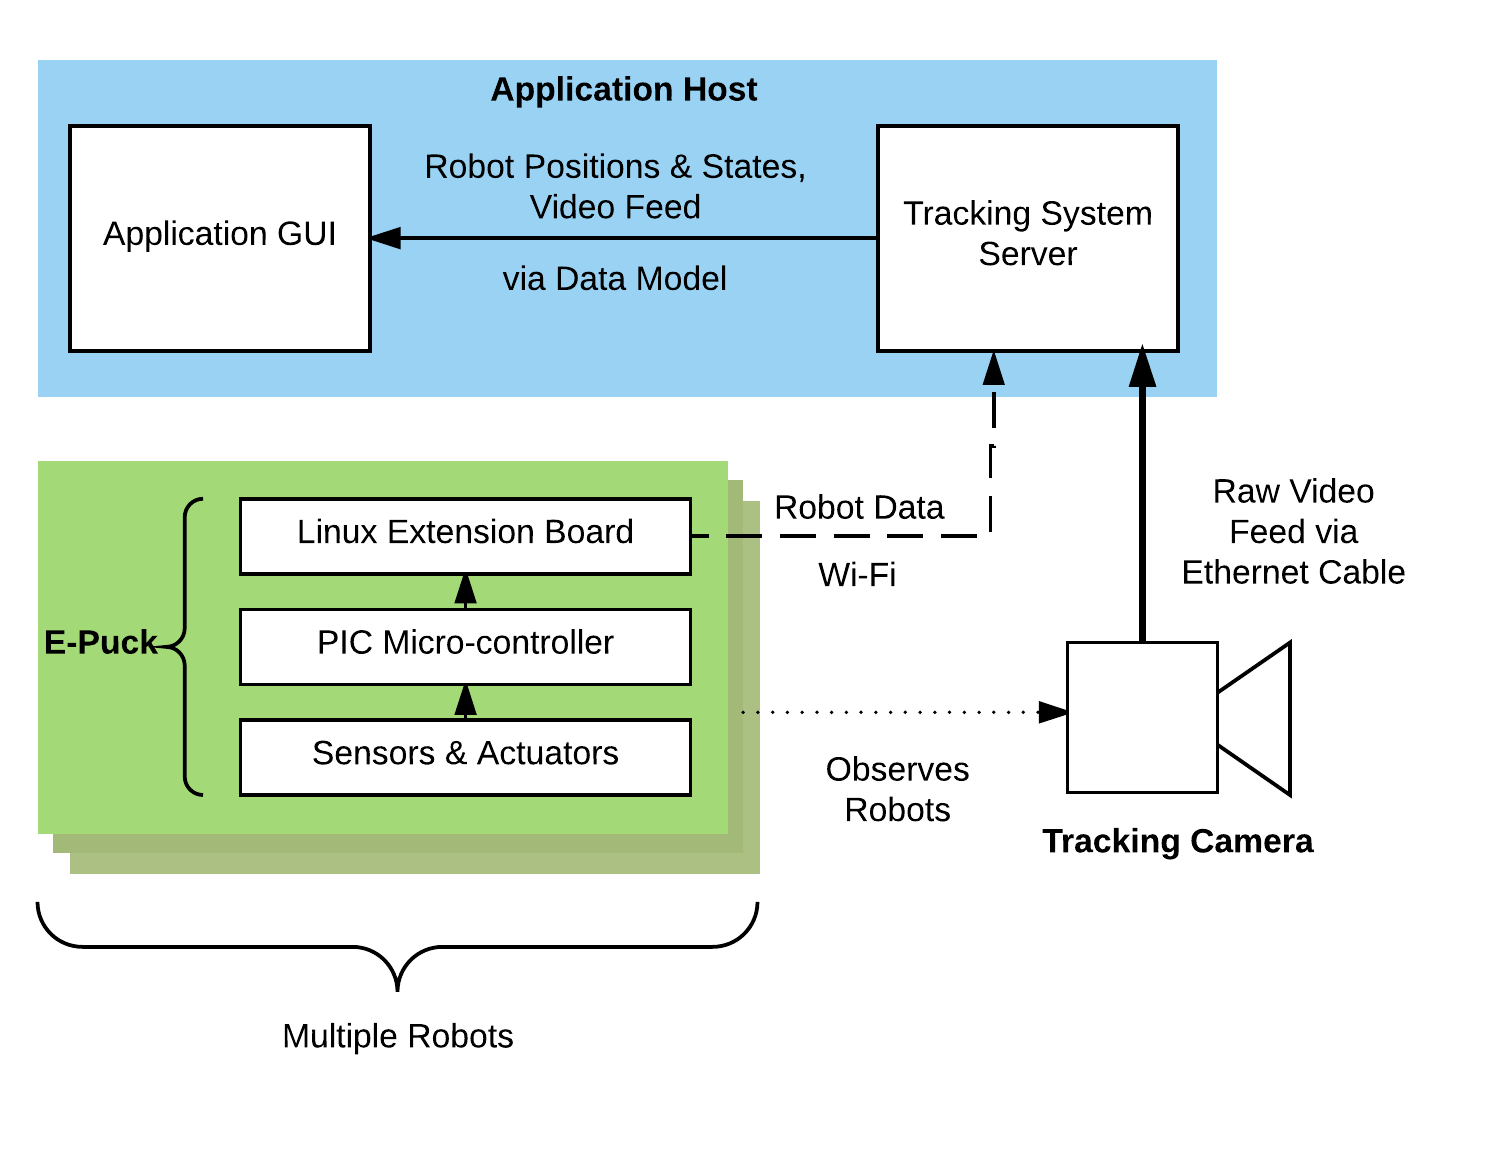
\includegraphics[scale=1.0]{SystemArchitecture.png}
	\caption{Expected general system architecture}
	\label{fig:SystemArchitecture}
	\end{center}
\end{figure}

\begin{multicols*}{2}

\section{Specification}
Given the aims stated above, a specification for the system to be developed can be stated as follows. The system:

\begin{enumerate}
	\item Must be comprised of a PC application.
	\item Must receive data related to the state of multiple robots.
	\item Must receive positional data for the same set of robots.
	\item Must receive a live video feed of the robots in their environment.
	\item Must collate this data and present it to the user in a combined graphical form.
	\item Must present auxiliary, non-spatial data to the user in textual or other forms.
	\item Must update in approximately real time.
	\item Must at minimum support the E-Puck swarm robotics platform.
	\item Should use a modularised structure.
	\item Should exchange data between modules using a platform-agnostic, extensible protocol.
	\item Should provide a basis for interoperability with a number of robotics platforms.
\end{enumerate}

\section{Literature Survey}
A number of key areas of literature have been identified as relevant to this project. A small body of work exists describing similar real time, graphical debugging systems for swarm and other robotics applications. These are primarily bespoke systems targeting single robotics platforms. More general work relating to human-swarm interaction, improvements to human-robot interaction through augmented reality (AR) tools, and swarm behaviour design theory are also considered.

\section{Project Plan}
\begin{thebibliography}{1}
\bibitem{SwarmIntelligence} Swarm intelligence. Dorigo M. Birattari M.
\end{thebibliography}

\end{multicols*}

\end{document}
